\chapter{Amplificadores Clase B}

\hspace{10pt}
El  circuito de la figura \ref{lab2_1} corresponde a un Amplificador
Clase B:


Diseñar el circuito teniendo en cuenta las siguiente
especificaciones:

\begin{enumerate}
	\item Fuente de alimentación simple. $V_{CC} = 18 V$.
	\item Carga $R_L= 8 \Omega$ .Diseñar para obtener la máxima potencia de salida posible (elegir
	los transistores de salida y disipadores necesarios).
	\item Impedancia de entrada $Z_i= 20K$.
	\item Ganancia de tensión de alterna. $\frac{\displaystyle v_o}{\displaystyle v_i}=19$.
	\item Frecuencia de corte en baja determinada por $C_L$ .  $f_{baja}=40
	Hz$.
	\item Asegurar que los capacitores $C_1$ y $C_2$ no influyan en la
	frecuencia de corte en baja.
	\item $C_F$ se coloca para  compensar el circuito. Se requiere
	que el cero esté a una frecuencia de 20 KHz.
	\item Realizar un cálculo teórico completo.
\end{enumerate}

Armar en un circuito de prueba el diseño realizado y efectuar las
siguientes mediciones manteniendo la llave S en 2:

\begin{enumerate}
	\item Verificar que variando $R_3$ se logra ajustar el punto de continua $V_{occ}$ a $\frac {\displaystyle V_{CC}}{\displaystyle 2}$.
	\item Excitar con un generador senoidal de amplitud variable a 1
	KHz. Visualizar la salida mediante un osciloscopio. Aumentar la amplitud
	de entrada hasta que se produzcan recortes. Reajustar el punto
	$V_{occ}$ para que el recorte sea simétrico. De producirse
	oscilaciones no deseadas tratar de eliminarlas colocando un
	capacitor de aproximadamente 1 nF entre colector y base de $Q_1$ y
	$Q_2$.
	\item Medir la ganancia de tensión utilizando el osciloscopio. Ingresar con una señal senoidal de 1 KHz
	, verificando que no se produzca recorte en la señal de salida.
	\item Ajustar la tensión de entrada de modo que la salida sea 10 $V_{pp}$ a 1
	KHz. En esta condiciones variar la frecuencia de entrada de manera
	de obtener las frecuencias de corte en baja y en alta.
	\item Mediante el método de medición con y sin carga estimar la impedancia de
	salida del amplificador.
	\item Visualizar la salida con la llave en 2 y en 1. Justificar las diferencias observadas.
\end{enumerate}

Realizar un informe completo del  laboratorio, comparando los
resultados obtenidos en la práctica con los calculados en forma
teórica.


\begin{figure}[h]
	\centering
	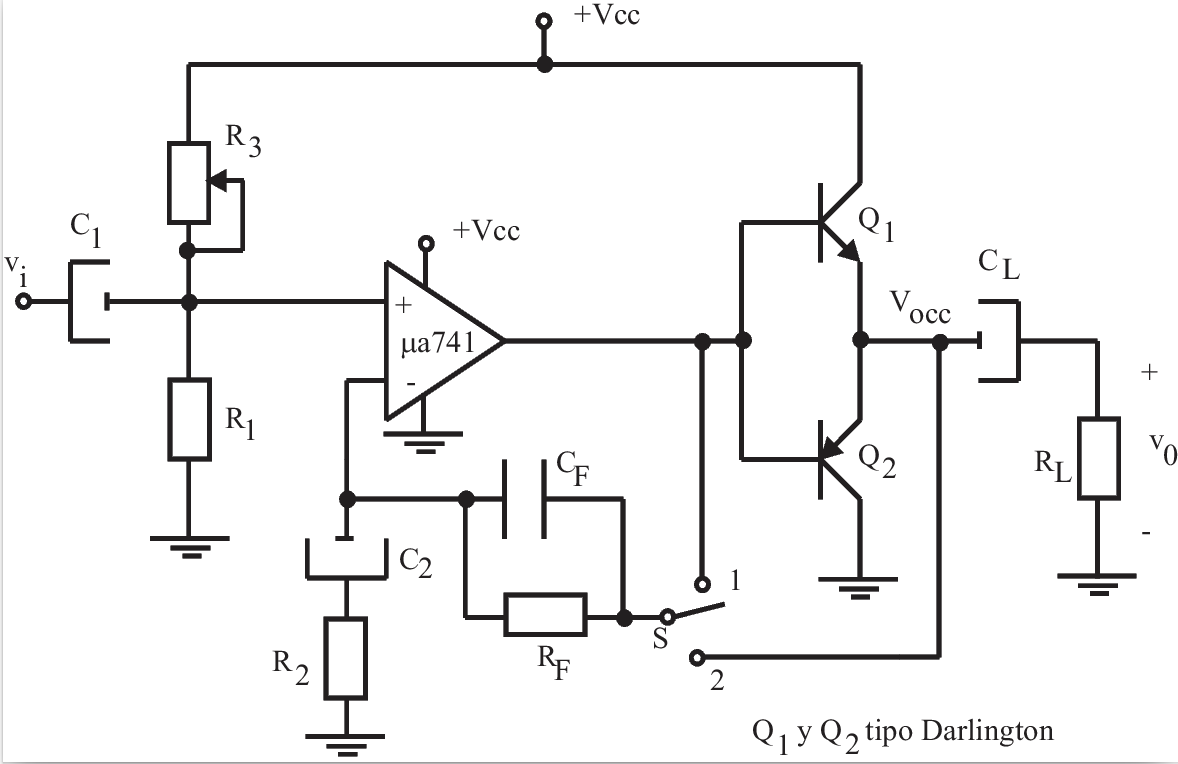
\includegraphics[width=0.8\linewidth]{figuras/lab2_1.png}\\
	\caption{}\label{lab2_1}
\end{figure}